\section{3. Modeling ET data}

In all previous steps, wrangling can be thought of as a condensing process, where the primary object is to remove, clean, and transform the data into a structure that is usable. However, once the data is put into tidy form, then the data must be transformed for specific visualizations and analyses. In this section, we think of \inlineR{all\_data\_cleaned} and \inlineR{all\_data\_tidy} as launching points to gain an understanding of our data \footnote{If you wish to start from here then read in the \inlineR{all\_data\_tidy} and \inlineR{all\_data\_cleaned} from cleaned data on OSF.}.

 Here, we are creating two data frames from \inlineR{all\_data\_tidy}: \inlineR{mem\_data} in L: 453 and \inlineR{gamm\_data} in L: 459. In general, maximally retaining informative columns is essential to creating a usable data frame. When building models, however, it is often best to remove variables that you will not be using. This is because some models can have complications interpreting unprocessed data types (e.g., \inlineR{NAs}). For \inlineR{mem\_data}, we start by selecting all necessary columns for the model (L: 454-455). Factor type conversion occurs next (L: 456). Finally, to get background information we join \inlineR{tidy\_quest\_data}. In addition to the \inlineR{mem\_data}, we create \inlineR{gamm\_data} by simply cloning \inlineR{mem\_data} in L: 459 and by adding a single variable needed in the GAMM models.

\lstinputlisting[style=mystyle, firstnumber=452]{scripts/chunk-All Data: Preparing for Models.R}

There are a handful of excellent papers that outline the advantages and disadvantages of different methods of eye-fixation analysis and relevant considerations for each method of analysis \parencite{Ito_Knoeferle_2022,Mirman_Dixon_Magnuson_2008,McMurray_2023,Barr_2008}. Here, we continue to focus on the data wrangling process and present the data wrangling steps--and decisions--needed to carry out two of the more widely used statistical analyses: generalized linear mixed effect models or GLMMs and generalized additive mixed effects models or GAMMs. Both GLMMs and GAMMs require specific contrast coding (e.g., dummy, orthogonal) of the data before running models to get expected results.  After contrast coding, all model building starts with maximal models, as justified by the design, working down to simpler models for model comparison. \parencite{Barr_Levy_Scheepers_Tily_2013}.
\newline
\subsection{3.1 GLMMs}
\subsection{3.1.1 GLMMs: coding}
For GLMMs coding, start with data type conversion (L: 464-465). Then, re-level both \inlineR{talker}(Native, Non-Native) and \inlineR{verb\_type}(Restrictive or Non-Restrictive) so that \inlineR{verb\_type}(Restrictive) and \inlineR{talker}-Native are both set as reference levels (L: 466-467).  We can then rename the contrasts to improve model output readability (L: 468-471) and later visualization. In L: 473 through L: 476, we normalize the \inlineR{time\_elapsed}. Lastly, we create a dataframe for the accent model (L:477).

\lstinputlisting[style=mystyle, firstnumber=463]{scripts/chunk-GLMM: Leveling the Data.R}

\subsection{3.1.2 GLMMs: models}

Two GLMMs were built using the \inlineR{lme4} package \parencite{Bates2014-eq}. Looks to the target (coded as 1, 0) served as the dependent variable. The \inlineR{Main Model} included three fixed effects: \inlineR{verb\_type} (Restrictive or Non-Restrictive), \inlineR{talker}(Native, Non-Native) and their interaction (L: 509). Random intercepts for \inlineR{subject\_img\_file},
\inlineR{Participant.Private.ID}, and
\inlineR{time\_normalized}.
 were included, as were random slopes for \inlineR{talker} and \inlineR{verb\_type}. The logit link function ("binomial") was specified in the model, equivalent to modeling logit-transformed response probability with identity link function. Model comparison \footnote{See \inlineR{AOW\_r\_work\_flow.rmd} for all model comparisons} showed preference for the full model with ANOVA comparisons (p < .001) and lower AIC and BIC. 

\lstinputlisting[style=mystyle, firstnumber=508]{scripts/chunk-GLMM: Main Model.R}

Similar to the above model, an accent only model was run on \inlineR{accent\_mem\_data}. Model specifications are identical to \inlineR{Main Model} outside of changing fixed effects to \inlineR{experience\_chinese} (L:540). Additionally, \inlineR{talker} is removed as a random slope because \inlineR{accent\_mem\_data} only has one \inlineR{talker}: accented. Full models were shown to outperform simpler models from  ANOVA comparisons (p < .001) and lower AIC and BIC, as well as non-convergence of simpler models. 

\lstinputlisting[style=mystyle, firstnumber=539]{scripts/chunk-GLMM: Accent Model.R}

\subsection{3.2 GAMMs}
GAMMs are becoming increasingly popular as they allow the researcher to model complex time course information without the need for assumptions of linearity. Like GLMM data, GAMM data must be first coded and prepared (L: 546-559). Here, we turn variables into factors and level them at the same time (e.g., L: 550-553). However, it is important to note that GAMMs do better with coded variables, L: 550-552. We create \inlineR{even} as a combination between conditions (L:554-555). Then we only \inlineR{select()} columns necessary for the analysis (L:557-559). Lastly, we split off the accent data for the accent GAMM (L: 560).

\lstinputlisting[style=mystyle, firstnumber=546]{scripts/chunk-GAMM: Leveling the Data.R}

GAMM Models were built using the \inlineR{mgcv} package \parencite{mgcv_wood_2017}. Model comparisons suggest that random intercept of \inlineR{Event} significantly improved maximal model. Like the GLMM model, the GAMM models treat target(L:603) as independent variable with dependent variables including: three fixed effects: \inlineR{talker\_coded} (L: 603), \inlineR{verb\_type\_coded} (L: 605) and their interaction (L: 607). Random effects included \inlineR{Event} (L: 612). Smooth terms were included for \inlineR{time\_elapsed} by levels of \inlineR{talker\_coded} (L: 604), \inlineR{verb\_type\_coded} (L: 606), and \inlineR{Condition} (L: 608). Smooth terms allow for a non-linear relationship between \inlineR{time\_elapsed} and the response variable \inlineR{verb\_type\_coded}, with a different smooth function for each level of variable (i.e., native/non-native). An additional smooth term for \inlineR{log\_SUBTLWF\_Obj} (L: 609) was included. Smooth terms for \inlineR{time\_elapsed} were included for grouping levels: \inlineR{Participant.Private.ID} and \inlineR{subject\_image\_file} (L:610-611). The logit link function ("binomial") was specified in the model, equivalent to modeling logit-transformed response probability with identity link function. 

\lstinputlisting[style=mystyle, firstnumber=602]{scripts/chunk-GAMM: Main Model.R}

The accent GAMM had identical structure to the main GAMM with the expectation of having only 1 main effect, \inlineR{experience\_chinese} (L: 642), and removing the smoothing term leveled by \inlineR{talker\_coded}. \inlineR{gamm\_data\_accented} was the data frame (L: 648). Model comparisons suggest that random intercept of \inlineR{Event} significantly improves in the maximum model.

\lstinputlisting[style=mystyle, firstnumber=641]{scripts/chunk-GAMM: Accent Model.R}

\subsection{3.3 Results}

 We observed nearly identical time course of predictive processing (Figure \ref{fig:smooth}) in which restricted sentences resulted in earlier looks to the target object than nonrestrictive sentences. Further, this effect is partially reduced in accented speech in a similar manner to \textcite{Porretta_et_al_2020}. For \inlineR{ggplot()} code and data wrangling for visualizations, see \inlineR{AOW\_r\_work\_flow.rmd}.

\begin{figure}[h]
    \centering
    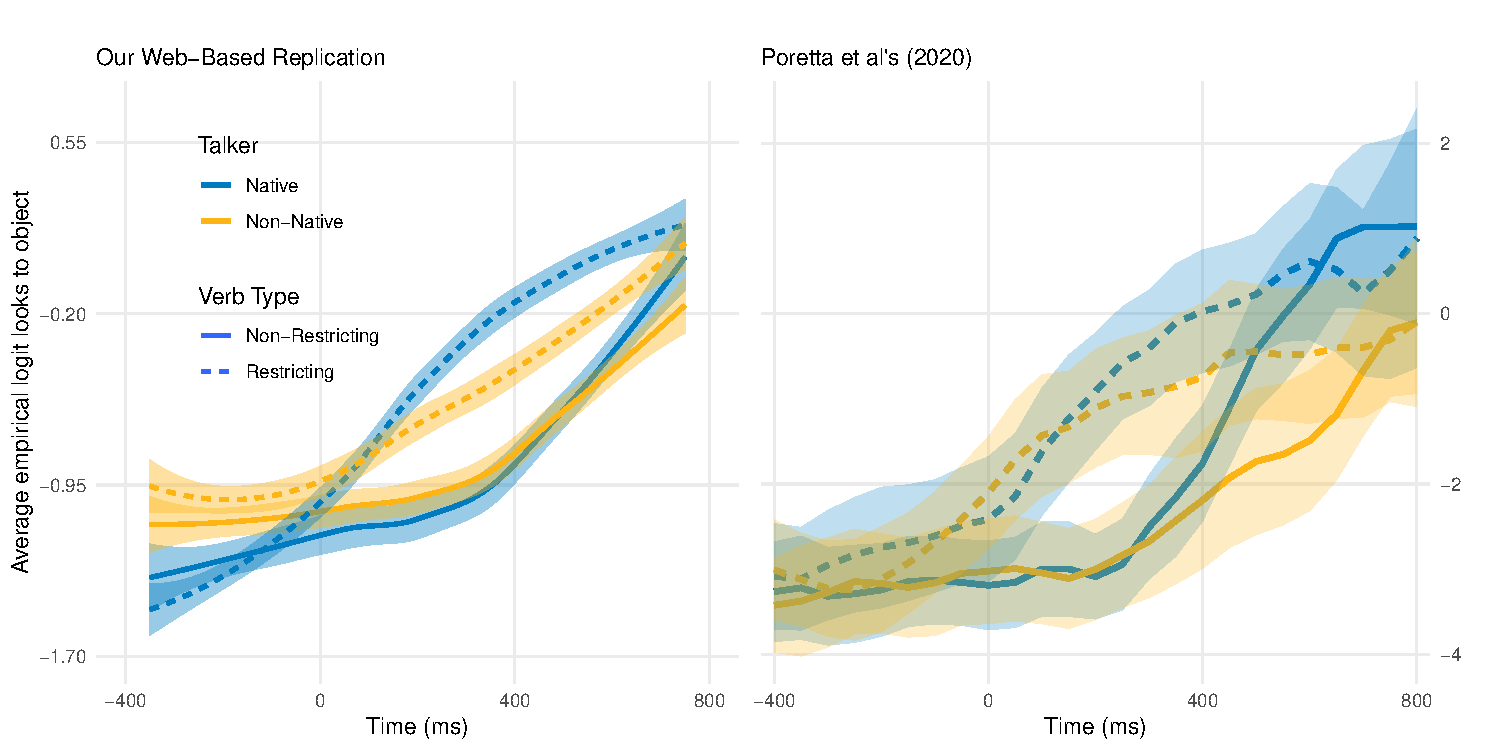
\includegraphics[width=\textwidth]{figures/smooth_comparison_plot.pdf}
    \caption{Left: our data. Right: \textcite{Porretta_et_al_2020}}
    \label{fig:smooth}
\end{figure}

\subsection{3.3.1 GLMM Results}
Results from the Main GLMM revealed a significant effect of  \inlineR{verb\_type}-Restricting  ($\beta$ = 0.281, SE = 0.067, z = 4.191, p < .001), indicating more looks to targets for restrictive \inlineR{verb\_type} over non-restrictive \inlineR{verb\_type}, see Figure \ref{fig:GLMM_cow_model} (left). Additionally, an interaction between speaker and verb type was found ($\beta$ = -0.136, SE = 0.053, z = -2.554, p = 0.011), indicating less looks when listening to the accented speaker. Results from the Accent GLMM found null results at an alpha-level of .05, see Figure \ref{fig:GLMM_cow_model} (right). 

\begin{figure}[H]
    \centering
    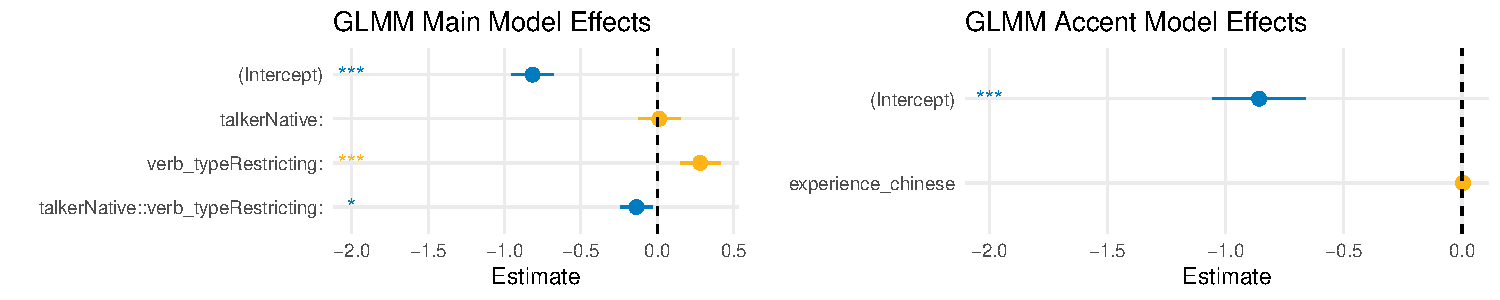
\includegraphics[width=\textwidth]{figures/GLMM_cow_model.pdf}
    \caption{Model output for parsimonious GLMM models}
    \label{fig:GLMM_cow_model}
\end{figure}

\subsection{3.3.2 GAMM Results}

Like the GLMM modeling results, results from the Main GAMM revealed a significant effect of  \inlineR{verb\_type}-Restricting  ($\beta$ = 0.398, SE = 0.129, z = 3.078, p = .002), indicating more looks to targets for restrictive \inlineR{verb\_type} over non-restrictive \inlineR{verb\_type}, see Figure \ref{fig:GAMM_cow_model} (left). Results from the Accent GAMM found null results at an alpha-level of .05. see figure \ref{fig:GAMM_cow_model} (right).

\begin{figure}[H]
    \centering
    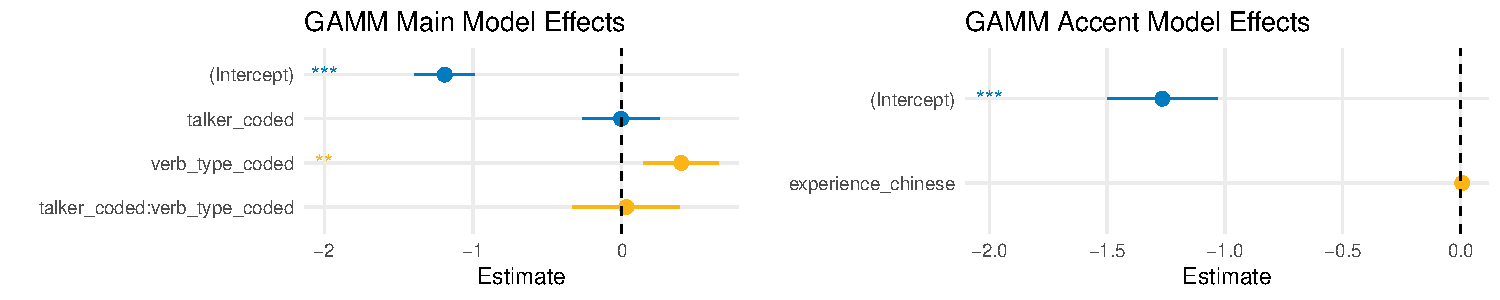
\includegraphics[width=\textwidth]{figures/GAMM_cow_model.pdf}
    \caption{Model output for parsimonious GAMM models}
    \label{fig:GAMM_cow_model}
\end{figure}
\newline
\newline